\subsubsubsection{biguint-add}

\begin{enumerate}
    \item \verb|Target|: Implement the addition of two biguints.
    \item \verb|Constraints logic|: 
        \begin{itemize}
            \item Equation for gates;
            \item Sumcheck between output and limbs;
            \item Rangecheck for limbs.
        \end{itemize}
    \item \verb|Circuit layout|: See \ref{fig:biguint-add-circuit-layout}.
    \item \verb|Trace layout|: See \ref{fig:biguint-add-trace-layout}.
    \item \verb|Constraints info and costs|
    \begin{itemize}
        \item gate type num: 1 (U32AddManyGate)
        \item gate ops num: limbs-num
        \item gate instance num: ceil(limbs-num / gate.ops)
        \item copy-constraints: limbs-num * 4
        \item max-degree: 4 (\verb|1 << limb-bits|)
    \end{itemize}
\end{enumerate}

\begin{figure}[!ht]
    \centering
    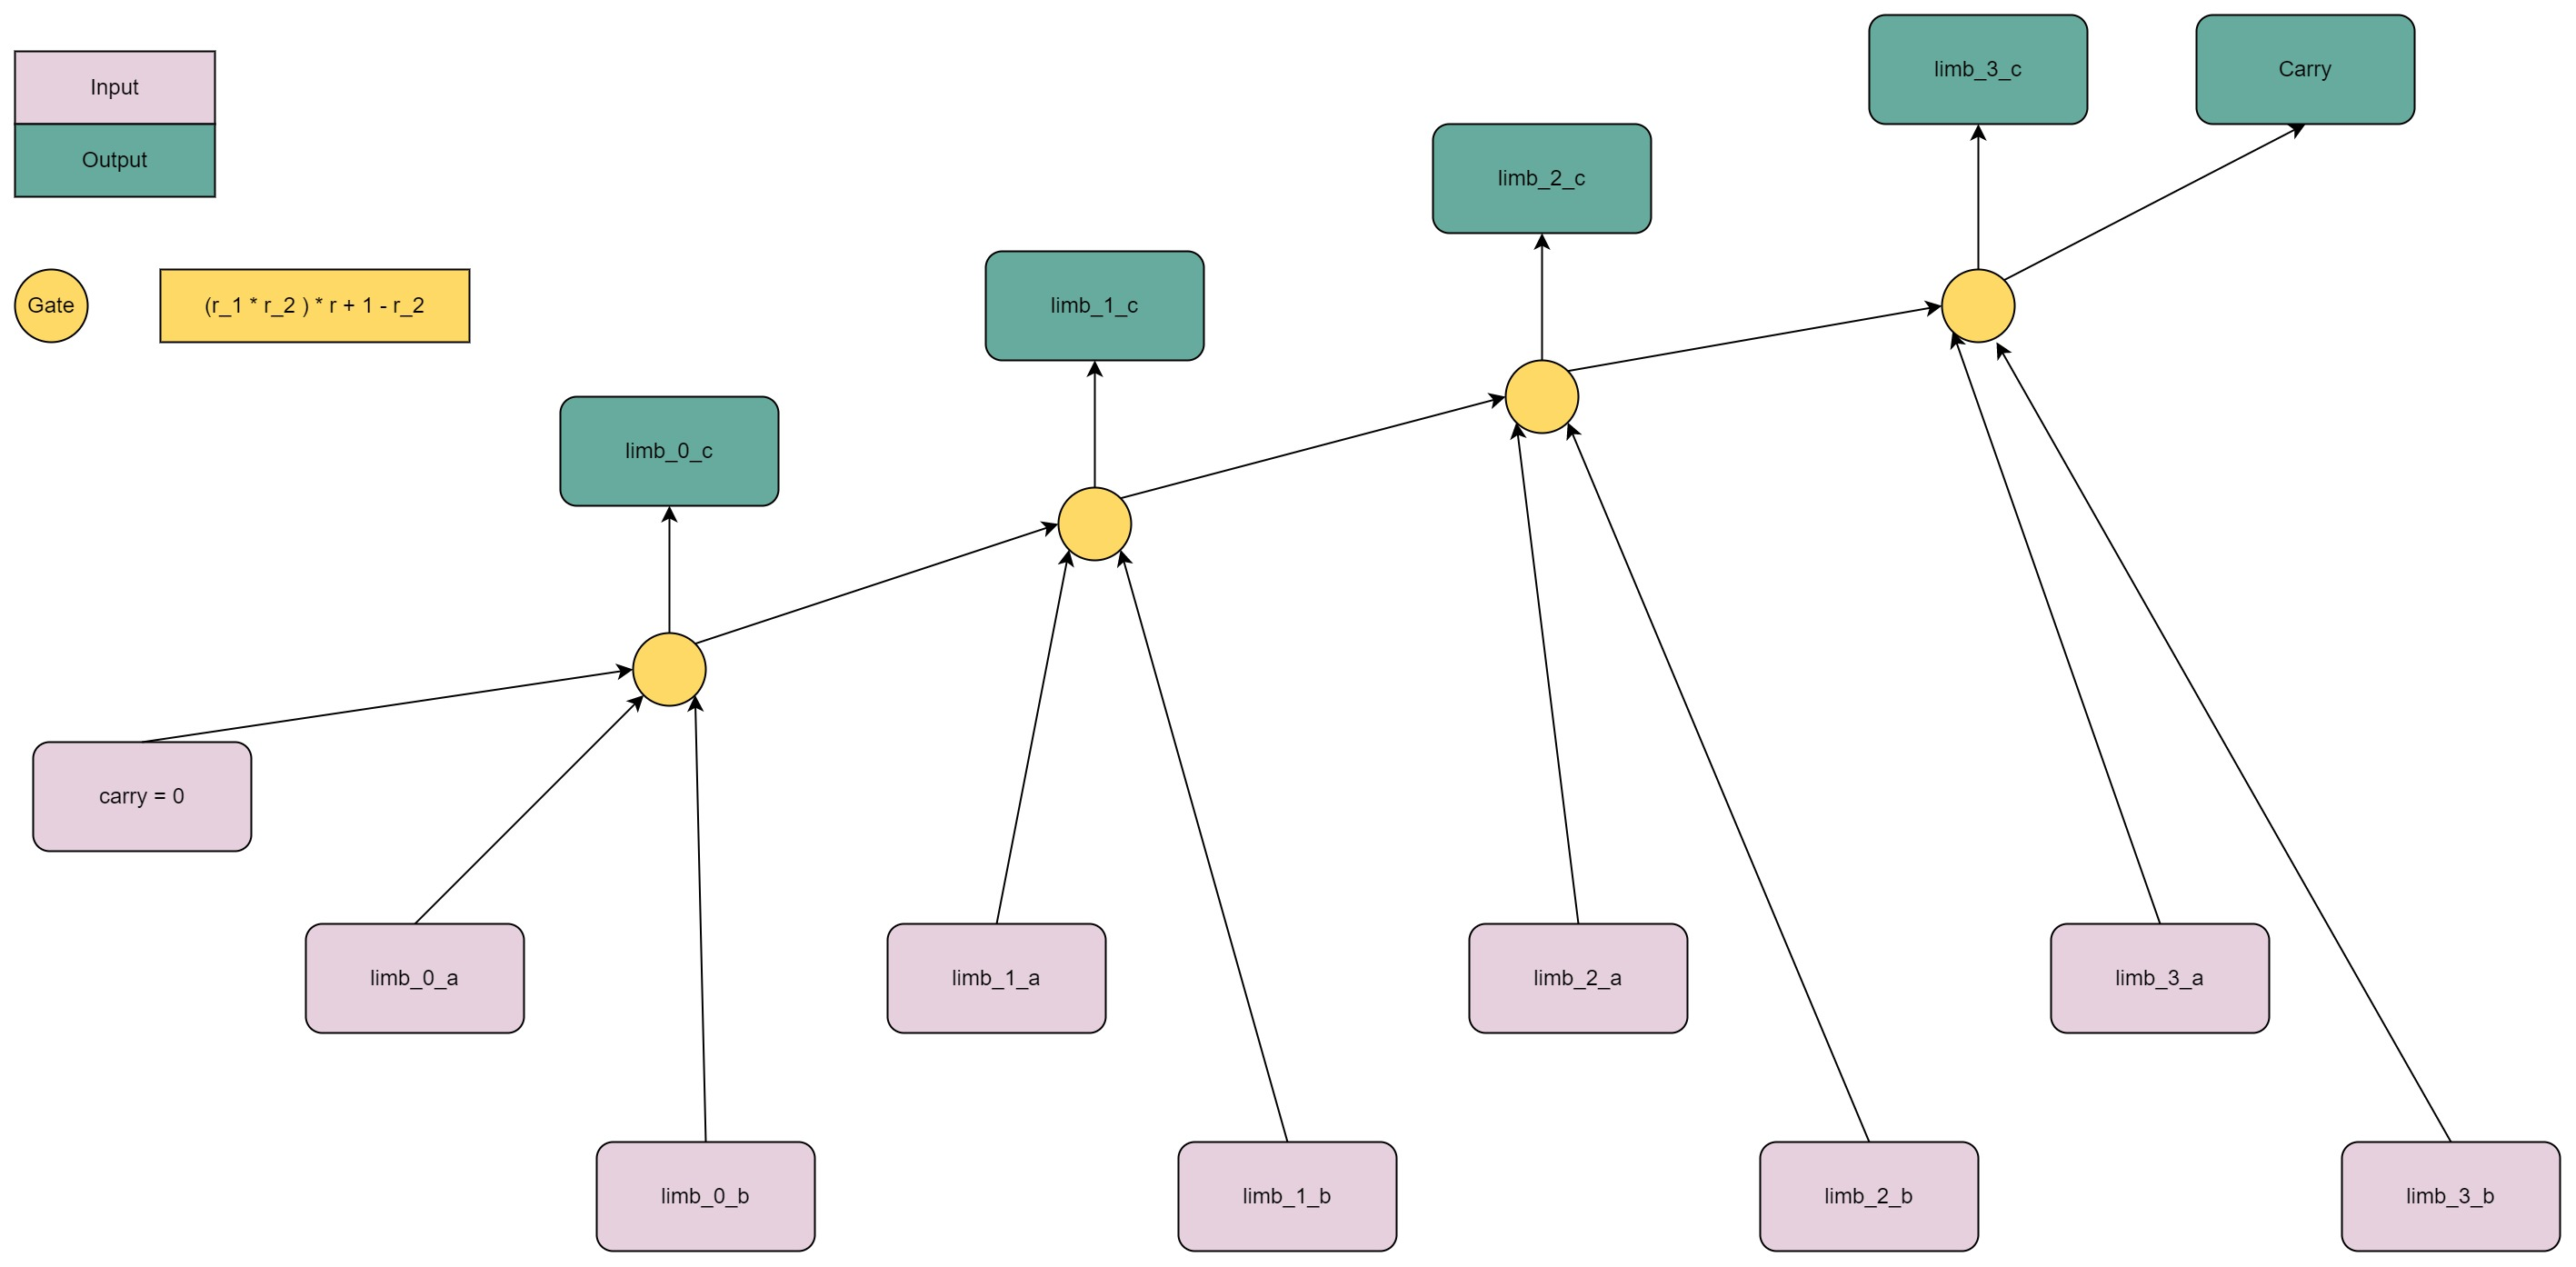
\includegraphics[width=0.6\textwidth]{biguint-add-circuit-layout.jpg}
    \caption{biguint-add circuit layout}
    \label{fig:biguint-add-circuit-layout}
\end{figure}
 
\begin{figure}[!ht]
    \centering
    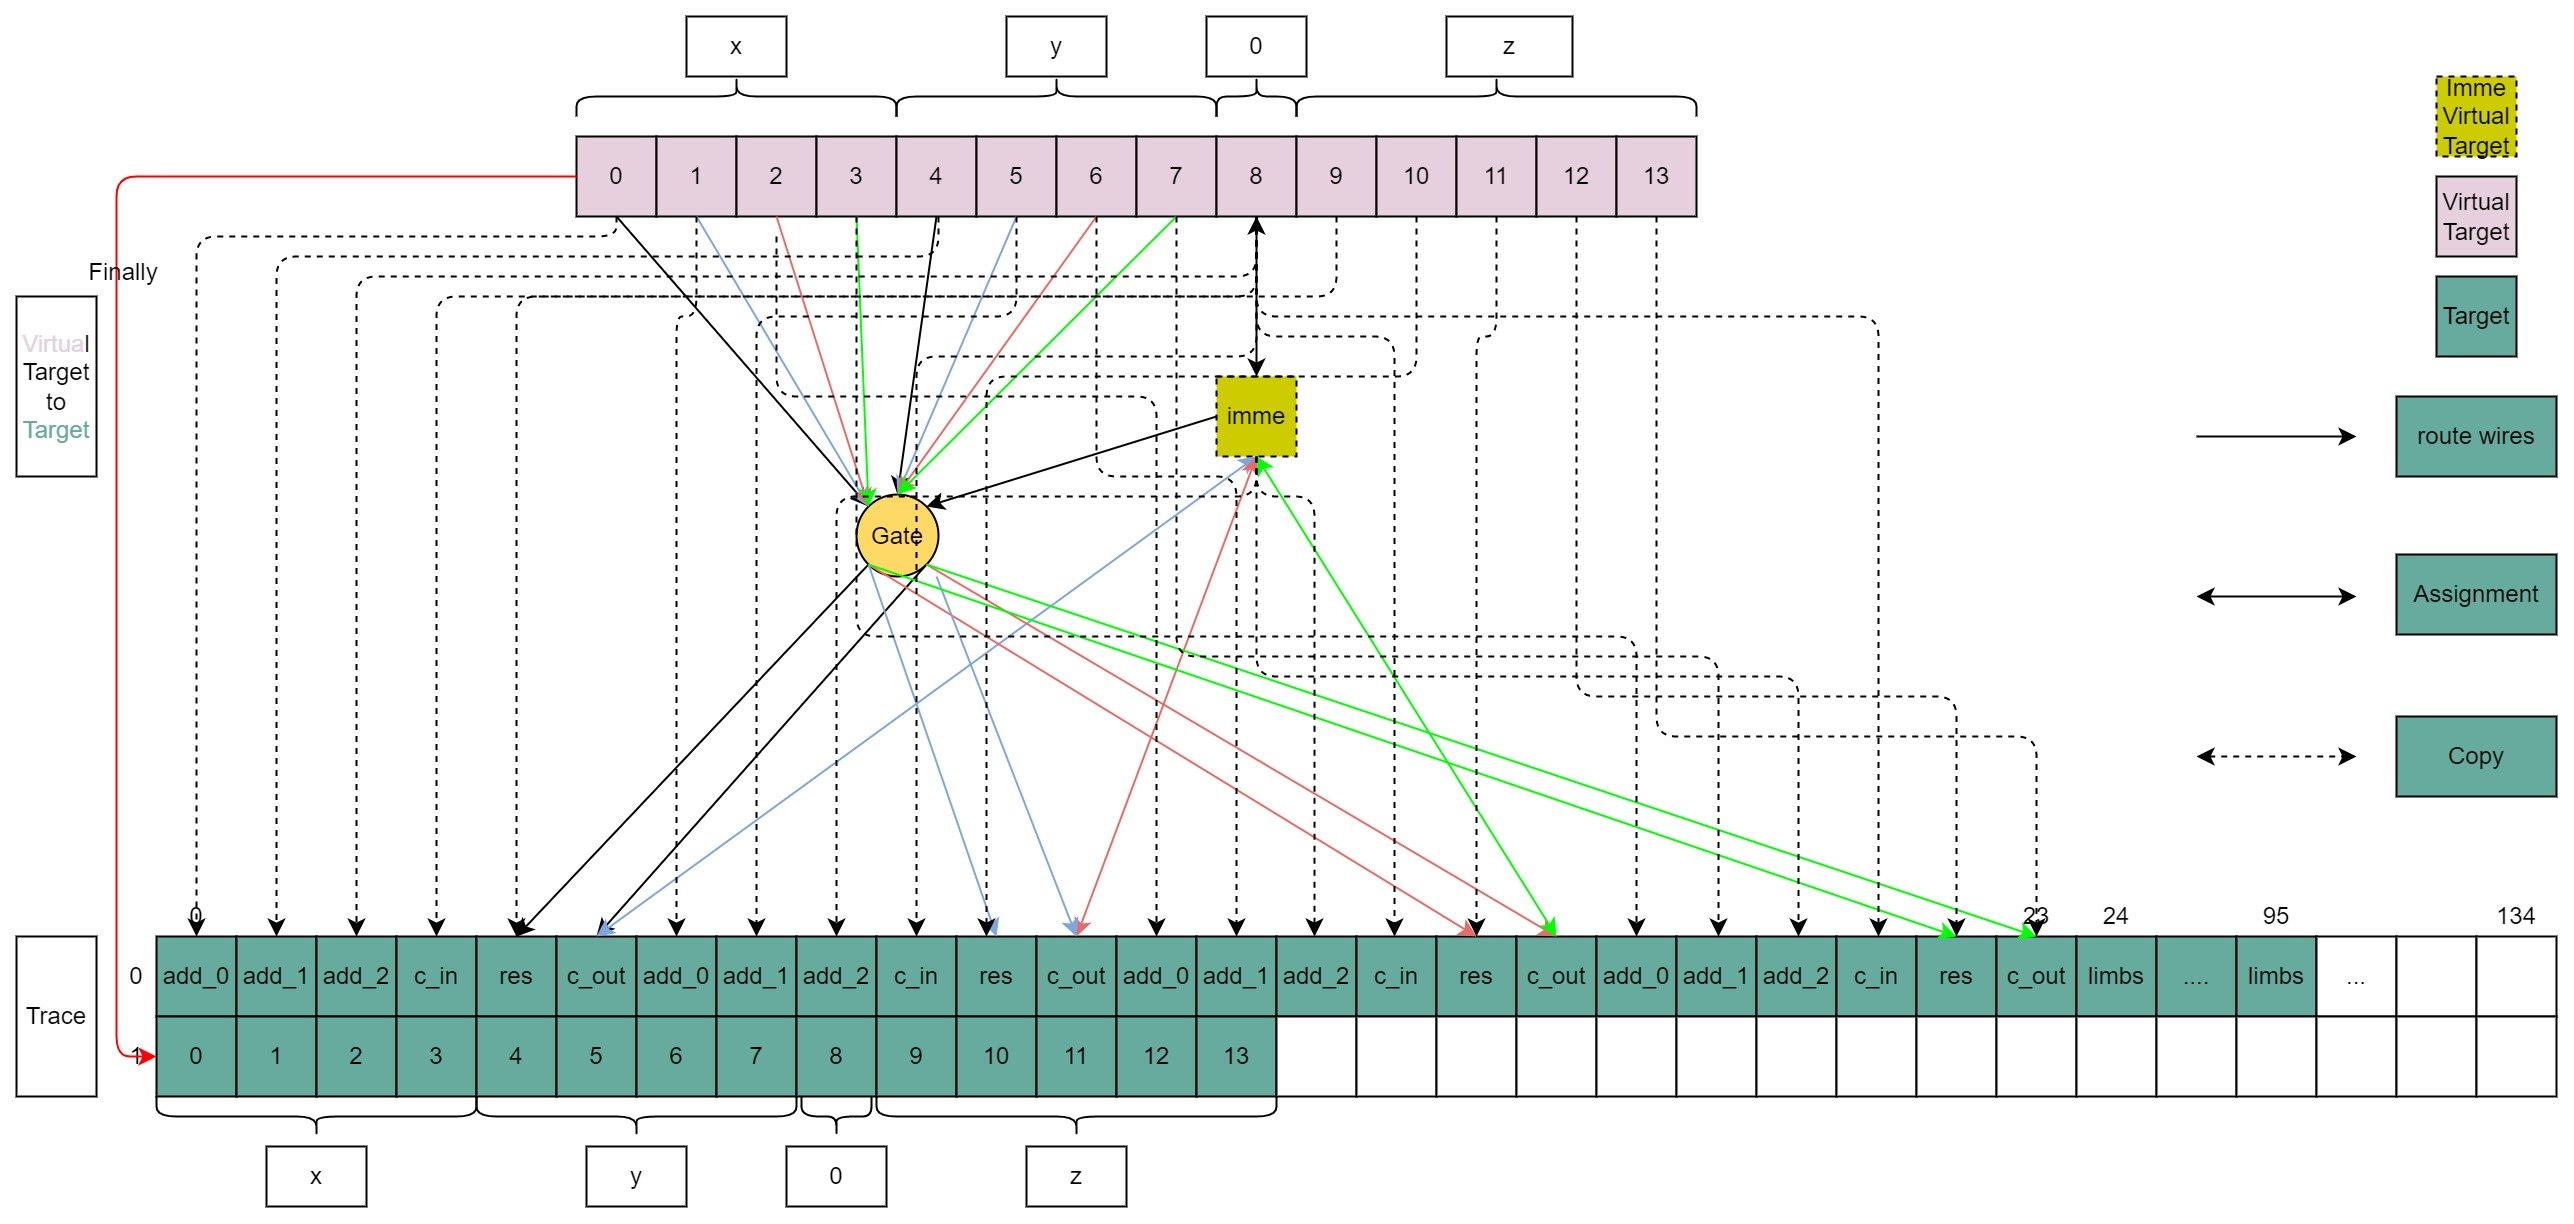
\includegraphics[width=0.6\textwidth]{biguint-add-trace-layout.jpg}
    \caption{biguint-add trace layout}
    \label{fig:biguint-add-trace-layout}
\end{figure}